% !TeX root = ../apuntes-ea.tex

\chapter{Aplicaciones prácticas}

En este capítulo se aplican las definiciones y teoremas generales dados en los capítulos anteriores para obtener teoremas más concretos. En gran medida, los teoremas que se plantean en esta sección están directamente relacionados con los ejercicios de la hoja 1.

\section{Ejemplos de grupos}

\subsection{Grupos infinitos}

\begin{ej}[Ejemplos de grupos infinitos]$ $\newline
	\begin{itemize}
		\item $(\R, +)$ es un grupo
		\item $(\R, \cdot)$ no es un grupo porque el $0$ no tiene inverso
		\item $(\R\setminus\{0\}, \cdot)$ es un grupo
		\item $(\R > 0, \cdot)$ es un grupo (subgrupo de $\R$)
		\item $(\R < 0, \cdot)$ no es un subgrupo porque no es cerrado
		\item $(\Z, +)$ es un grupo
		\item $n\Z = \{\dots, -2n, -n, 0, n, 2n, \dots\}$ con la suma es un grupo
		\item $GL_2(\R) = \{A \in R^{2\times 2} \mid \det A \neq 0\}$ las matrices reales no singulares $2\times 2$ forman un grupo con el producto
		\item Por lo anterior, las aplicaciones lineales que tienen inversa forman un grupo con la composición (componer aplicaciones es lo mismo que multiplicar matrices y la inversa existe $\iff \det A \neq 0$)
	\end{itemize}
\end{ej}

\subsection{Grupos finitos.}

\begin{ej}[Grupo de las clases módulo $n$]
	$\ZnZ = \{\overline{0}, \overline{1}, \overline{2}, \dots, \overline{n-1}\}$ con la suma es un grupo.
\end{ej}

\begin{ej}
	El conjunto $(\Z^*/n\Z, \cdot)$ formado por $\{1, 2, \dots, n\}$ con el producto no da un grupo, porque hay elementos que no tienen inverso. Es interesante considerar el conjunto de unidades en este conjunto:
	
	\begin{align*}
		\uds{\Z^*/n\Z} = \{a \in \Z^*/n\Z \mid \exists \inv{a}, a \inv{a} = 1\}
	\end{align*}
	
	que sí es un grupo con el producto.
\end{ej}

\begin{ej}[Grupo de cuaterniones]
	\label{ej:grupocuaterniones}
	Llamamos $H$ al subgrupo de $GL_2(\mathbb{C})$ generado por $A$ y $B$: $H = \langle A, B\rangle$ donde 
	\begin{align*}
	A = \left(\begin{array}{cc}
	0 & 1 \\ -1 & 0
	\end{array}\right),\ B = \left(\begin{array}{cc}
	0 & i \\ i & 0
	\end{array}\right)
	\end{align*}
	De probar las multiplicaciones de $A$ y de $B$ consigo mismas y entre ellas se obtiene la presentación.
	\begin{align*}
	o(A) = o(B) = 4\quad A^2 = B^2 \quad BA = AB^3
	\end{align*}
	y queda que $H = \{1, B, B^2, B^3, A, AB, AB^2, AB^3\}$. Es posible obtener cualquier operación de $A$ y $B$ a partir de la presentación.
	
	\begin{figure}[h]
		\centering
		\begin{tabular}{c|cccccccc}
			elemento & $1$ & $B$ & $B^2$ & $B^3$ & $A$ & $AB$ & $AB^2$ & $AB^3$ \\ \hline
			orden   &  1  &  4  &   2   &   4   &  4  &  4   &   4    &   4
			% TODO: completar los órdenes
		\end{tabular}
		\caption{Órdenes de los elementos de $H$}
	\end{figure}
\end{ej}

\begin{ej}[El famoso grupo $D_4$]
	\label{ej:famosogrupod4}
	$D_4$ es el grupo formado por las composiciones de rotaciones y simetrías que llevan un cuadrado en un cuadrado ($f(\square) = \square$). También se llama grupo diédrico de órden $4$.
	\begin{figure}[h]
		\centering
		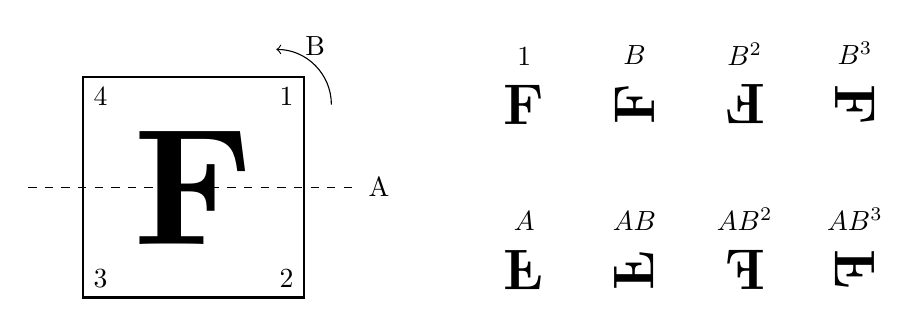
\begin{tikzpicture}[scale=0.7]
		
		% giro
		\draw[->] (2.5,1.5) arc (0:90:1cm) node[midway, above] {B};
		
		% simetría
		\draw[dashed] (-3,0) -- (3,0) node[pos=1,right] {A};
		
		% cuadrao
		\draw[thick] (2,2) node[anchor=north east] {1} --
		(2,-2) node[anchor=south east] {2} --
		(-2,-2) node[anchor=south west] {3} --
		(-2, 2) node[anchor= north west] {4} -- cycle;
		
		\draw (0,0) node {\scalebox{6}{\textbf{F}}};
		
		% las efes
		% las efes: los giros
		\begin{scope}[shift={(6,0)}]
		\draw (0, 1.5) node[label={$1$}] {\huge \textbf{F}};
		\draw (2, 1.5) node[label={$B$}] {\rotatebox{90}{\huge \textbf{F}}};
		\draw (4, 1.5) node[label={$B^2$}] {\rotatebox{180}{\huge \textbf{F}}};
		\draw (6, 1.5) node[label={$B^3$}] {\rotatebox{270}{\huge \textbf{F}}};
		
		% las efes: la simetrías de los giros
		\draw (0, -1.5) node[label={$A$}] {\scalebox{1}[-1]{\huge \textbf{F}}};
		\draw (2, -1.5) node[label={$AB$}] {\rotatebox{90}{\scalebox{1}[-1]{\huge \textbf{F}}}};
		\draw (4, -1.5) node[label={$AB^2$}] {\rotatebox{180}{\scalebox{1}[-1]{\huge \textbf{F}}}};
		\draw (6, -1.5) node[label={$AB^3$}] {\rotatebox{270}{\scalebox{1}[-1]{\huge \textbf{F}}}};
		\end{scope}
		\end{tikzpicture}
		\label{fig:d4geometria}
		\caption{Simetría $A$ y rotación $B$ que compuestas forman los elementos del grupo $D_4$}
	\end{figure}
	
	Geométricamente,
	\begin{align*}
	A = \left(\begin{array}{cc}
	1 & 0 \\ 0 & -1
	\end{array}\right), \qquad B = \left(\begin{array}{cc}
	\cos \alpha & -\sin \alpha \\ \sin \alpha & \cos \alpha
	\end{array}\right),\quad \alpha = \frac{\pi}{2}
	\end{align*}
	pero una vez hemos comprobado que todas las posibles operaciones $A^iB^j$ y $B^iA^j$ quedan dentro del grupo (que es cerrado), que existe el neutro (la identidad) y que cada elemento tiene su inverso, podemos obviar el significado geométrico y pasar a describirlo mediante la presentación del grupo.
	\begin{align}
	\label{eq:presentacionD4}
	D_4 = \langle A, B \rangle \text{ donde } o(A) = 2,\ o(B) = 4, BA = AB^3
	\end{align}
	y además queda que $D_4 = \{1, B, B^2, B^3, A, AB, AB^2, AB^3\}$.
	
	\begin{figure}[h]
		\centering
		\begin{tabular}{c|cccccccc}
			elemento & $1$ & $B$ & $B^2$ & $B^3$ & $A$ & $AB$ & $AB^2$ & $AB^3$ \\ \hline
			orden   &  1  &  4  &   2   &   4   &  2  &  -   &   -    &   -
			% TODO: completar los órdenes
		\end{tabular}
		\caption{Órdenes de los elementos de $D_4$}
	\end{figure}
	
	\textbf{Nota:} lo que hemos hecho con un cuadrado también se puede hacer con un triángulo.
\end{ej}

\begin{ej}[Grupo de biyecciones $S_3$]
	Ver figura \ref{fig:s3elemento12}. Llamamos $S_3$ al grupo de las biyecciones $f:\{1,2,3\} \to \{1,2,3\}$. También podemos pensar en este grupo como el grupo de las permutaciones de 3 elementos. De hecho, utilizamos la siguiente notación para las biyecciones de $S_3$:
	\begin{itemize}
		\item $(1)$ indica que $f(1) = 1$. Por defecto, $f(2) = 2$ y $f(3) = 3$.
		\item $(12)$ indica que $f(1) = 2$ y $f(2) = 1$. Por defecto $f(3) = 3$.
		\item $(123)$ indica que $f(1) = 2,\ f(2) = 3,\ f(3) = 1$.
		\item $(13)$ indica que $f(1) = 3,\ f(3) = 1$ y por defecto $f(2) = 2$.
	\end{itemize}
	
	\begin{figure}[h]
		\centering
		\begin{tikzpicture}[scale=0.6]
		\node (1) at (0,1) {$1$};
		\node (2) at (0,0) {$2$};
		\node (3) at (0,-1) {$3$};
		
		\node (f1) at (3,1) {$1$};
		\node (f2) at (3,0) {$2$};
		\node (f3) at (3,-1) {$3$};
		
		\draw (0,0) ellipse (.7 and 2);
		\draw (3,0) ellipse (.7 and 2);
		
		\draw[-{Latex[length=2mm]}] (1) -- (f2);
		\draw[-{Latex[length=2mm]}] (2) -- (f1);
		\draw[-{Latex[length=2mm]}] (3) -- (f3);
		\end{tikzpicture}
		\caption{Elemento (12) de $S_3$}
		\label{fig:s3elemento12}
	\end{figure}
	
	En este grupo ocurre algo parecido a lo que ocurre en $D_4$. Sea $a = (123), b = (12)$. Podemos presentar el grupo con
	\begin{align}
	S_3 = \langle a, b\rangle\text{ donde } o(a) = 3,\ o(b) = 2,\ ba = ab^2
	\end{align}
	y por tanto $S_3 = \{1, a, a^2, b, ab, a^2b\} = \{(1), (12), (13), (23), (123), (132)\}$. %TODO comprobar
\end{ej}

\section{Clasificación de grupos finitos}

Vamos a aplicar el teorema \ref{thm:noprobado1} a grupos abelianos.

\begin{thm}
	Sea $G$ abeliano con $|G| = p_1^{\alpha_1}p_2^{\alpha_2}\dots p_n^{\alpha_n}$. Entonces
	\begin{align}
	G \isom \Z/p_1^{\beta_{11}}\Z \times \Z/p_1^{\beta_{1s_1}}\Z \times \dots \Z/p_n^{\beta_{n1}}\Z \times \Z/p_1^{\beta_{ns_n}}\Z \text{ donde } \alpha_i = \sum_{j = 1\dots s_i} \beta_{ij}
	\end{align}
\end{thm}

En particular, se cumple que para grupos cíclicos $G$ de orden $n$, donde $G \isom \ZnZ$.

\begin{thm}
	\label{thm:znzisomproductodirecto}
	Sea un número y su factorización en primos: $n = p_1^{\alpha_1}p_2^{\alpha_2}\dots p_n^{\alpha_n}$. Entonces
	\begin{align}
	\ZnZ \isom \Z/p_1^{\alpha_1}\Z \times \Z/p_2^{\alpha_2}\Z \times \dots \times \Z/p_n^{\alpha_n}\Z
	\end{align}
\end{thm}

\begin{proof}
	Sea $d$ tal que $d \divides n$ y $n = dn'$. Por tanto $n' = p_2^{\alpha_2}\dots p_n^{\alpha}$ y $d = p_1^{\alpha_1}$. Como $\ZnZ = \{0, 1, 2, \dots, n', \dots, n-1\}$ tenemos que $o(n') = p_1^{\alpha_1}$. Luego $H = \langle n' \rangle$ es el único subgrupo de orden $p_1^{\alpha_1}$ y $N = \langle p_1^{\alpha_1} \rangle$ es el único subgrupo de orden $n'$. Ahora bien, por cómo hemos elegido $n'$ y $d$, $mcd(n', d) = 1$ por lo que $\ZnZ \isom \Z/d\Z \times \Z/n'\Z$. Podemos repetir este procedimiento hasta que descompongamos $n$ en potencias de primos y tendremos que $mcd(p_1^{\alpha_1}, p_2^{\alpha_2}, \dots, p_n^{\alpha_n}) = 1$ y por tanto $\ZnZ \isom \Z/p_1^{\alpha_1}\Z \times \Z/p_2^{\alpha_2}\Z \times \dots \times \Z/p_n^{\alpha_n}\Z$
\end{proof}

Lo que nos dice este teorema es que si un grupo es cíclico de orden $n$ entonces es isomorfo a $\ZnZ$ y a su vez a un producto directo en el que cada uno de los factores tiene como orden un factor de $n$, sin separarlos con la multiplicidad.

\begin{ej}
	Si un grupo de orden $12$ es cíclico entonces es isomorfo a $\Z/4\Z \times \Z/3\Z$, y no es isomorfo a $\Z/2\Z \times \Z/2\Z \times \Z/3\Z$.
\end{ej}

\begin{thm}
	Sea $G$ abeliano donde $|G| = r\cdot s$ con $mcd(r,s) = 1$ y ean $K < G \land N < G$ donde $|K| = r \land |N| = s$. Entonces $G \isom K \times N$.
\end{thm}

\begin{proof}
	Sabemos que $f:K\times N \to G,\ (k, h) \mapsto kh$ es un homomorfismo y por tanto $\ima f < G$. Para probar que $f$ es un isomorfismo probaremos que $\ima f = G$. Como $|K| = r \land |N| = s$ y $r$ y $s$ son coprimos entonces $K \cap N = \{e\}$. Por tanto $|K \cap N| = 1$ y utilizando el teorema \ref{thm:cardinalidadproductolibre} tenemos que $|KN| = \frac{|K||N|}{|K \cap N|} = |K| |N| = rs$ por lo que $f$ es sobreyectiva, y, por tanto, biyectiva, es decir, que $f$ es un isomorfismo.
\end{proof}

\begin{ej}
	Podemos afirmar que si $|G| = 6$ y $G$ es abeliano entonces $G \isom \Z/6\Z \isom \Z/2\Z \times \Z/3\Z$.
\end{ej}

Observemos que la hipótesis de abeliano es fundamental (ver ejemplo \ref{ej:nohomoentreproducto}).

\subsection{Teorema de clasificación de grupos finitos de orden pequeño}

\label{gruposfinitosnotables}

\begin{thm}[Grupos notables de distintos órdenes finitos.]$ $\newline
 \label{thm:clasificacionfinitos}
	
	\begin{itemize}
		\item $|G| = 3, 5, 7, 11 \dots, p$ donde $p$ es primo:
		\begin{itemize}
			\item Abelianos cíclicos: son isomorfos con $\Z/p\Z$.
			\item Abelianos no cíclicos: no hay, por el corolario del teorema de Lagrange \ref{thm:lagrange}.
		\end{itemize}
		\item $|G| = 4$:
		\begin{itemize}
			\item Abelianos cíclicos: son isomorfos con $\Z/4\Z$
			\item Abelianos no cíclicos: son isomorfos con $\Z/2\Z \times \Z/2\Z$.
			\item No abelianos: no hay.
		\end{itemize}
		\item $|G| = 6$:
		\begin{itemize}
			\item Abelianos cíclicos: son isomorfos con $\Z/6\Z$.
			\item Abelianos no cíclicos: no hay porque todo grupo abeliano cuyo orden se puede descomponer en dos primos es cíclico (ver Hoja 1 ejercicio 19).
			\item No abelianos: todos son isomorfos con $D_3 \isom S_3$ (ver ejemplo \ref{ej:orden6noabisomd3}).
		\end{itemize}
		\item $|G| = 8$:
		\begin{itemize}
			\item Abelianos cíclicos: son isomorfos con $\Z/8\Z$.
			\item Abelianos no cíclicos: son isomorfos o bien con $\Z/4\Z \times \Z/2\Z$ o bien con $\Z/2\Z \times \Z/2\Z \times \Z/2\Z$ (depende de los órdenes de los elementos de $G$).
			\item No abelianos: son isomorfos o bien con el famoso grupo $D_4$ (ver ejemplo \ref{ej:famosogrupod4}) o bien con el grupo de cuaterniones $H$ (ver ejemplo \ref{ej:grupocuaterniones}). Ver ejemplo \ref{ej:orden8noabisom}
		\end{itemize}
	\end{itemize}
	
\end{thm}

\begin{proof}
	En lo que resta de sección se dan algunos ejemplos de los razonamientos que llevan a estas afirmaciones.
\end{proof}

\begin{ej}
	\label{ej:orden6noabisomd3}
	Sea $G$ no abeliano con $|G| = 6$. Entonces $G \isom D_3$.
\end{ej}

\begin{proof}
	\begin{enumerate}
		\item $G$ no abeliano $\implies G$ no cíclico $\implies \exists g \in G \mid o(g) \neq 6$
		\item $G$ no abeliano $\implies \exists b \in G \mid o(b) \neq 2 \implies o(b) = 3$ ya que si $b \in G$ entonces $o(b) \divides |G|$ (corolario teorema de Lagrange (\ref{thm:lagrange})).
		\item Sabemos pues que $\langle b \rangle = \{1, b, b^2\} < G$ y $|\langle b \rangle| = 3 \implies [G:\langle b \rangle] = \frac{|G|}{|\langle b \rangle|} = 2$. Es decir, que hay otra caja disjunta en la partición a la que llamamos $K$
		\item Por el teorema del cardinal del producto libre (teorema \ref{thm:cardinalidadproductolibre}) tenemos que $6 \geq |HK| = \frac{|H||K|}{|\langle b \rangle \cap K}$. Como $\langle b \rangle \cap K = \{e\}$ por ser las cajas disjuntas tenemos que $|K| = 2$ ya que si fuera $|K| = 3$ tendríamos que $|HK| = 9 \not \leq 6$.
		\item Definimos $\phi_a(x) : G \to G,\ x \mapsto ax\inv{a}$ (el isomorfismo de conjugación). $\phi_a$ es un isomorfismo, incluso cuando lo restringimos a un subgrupo normal. El subgrupo $\langle b \rangle$ es normal porque tiene índice 2 (ver teorema \ref{thm:indice2normal}).
		\item Por ello tenemos que si $\phi_a(x) = y$ entonces tiene que ser $o(x) = y$. Por tanto, aplicando $\phi_a$ a $b$ tenemos lo siguiente:
		\begin{align*}
		\phi_a(b) = ab\inv{a} = b \implies ab = ba \implies G \text{ abeliano} \\
		\phi_a(b) = ab\inv{a} = \inv{b} \implies ab = b^2a \implies ba = ab^2
		\end{align*}
		\item La primera no puede ser por hipótesis. La segunda nos da el final de la presentación de $D_3$:
		\begin{align*}
		D_3 = \langle a, b \rangle \text{ donde } o(a) = 2,\ o(b) = 3,\ ba = ab^2
		\end{align*}
	\end{enumerate}
\end{proof}

\begin{ej}
	\label{ej:orden8noabisom}
	Probar que si $G$ es un grupo no abeliano con $|G| = 8$ entonces o bien $G \isom D_4$ o bien $G \isom H$ donde $H$ es el grupo de cuaterniones (ver ejemplo \ref{ej:grupocuaterniones}).
\end{ej}

\begin{proof}$ $\newline
	\begin{enumerate}
		\item Tenemos que $G$ no es abeliano. Por el contrarrecíproco del teorema \ref{thm:ciclicoimplicaabeliano} tenemos que no puede ser cíclico por lo que $\not\exists g \in G \mid o(g) = 8$.
		\item Por el teorema \ref{thm:abelianosdeorden2} sabemos que $\exists b \in G \mid o(b) \neq 2 \implies \mathbf{o(b) = 4}$.
		\item Por el teorema de Lagrange \ref{thm:lagrange} sabemos que dicho $b$ tiene que tener $o(b) = 4$ ya que $\forall b \in G, o(b) \divides |G|$. Por tanto $\langle b \rangle = \{1, b, b^2, b^3\}$.
		\item Como $\langle b \rangle$ tiene orden $4$, el índice es $[G: \langle b \rangle] = 2$ por lo que hay otro subgrupo en $G$ disjunto a $\langle b \rangle$. Sea $a$ un elemento de dicho subgrupo.
		\item Fijado $a$, definimos el isomorfismo de conjugación $\phi_a: G \to G,\ \phi_a(x) = ax\inv{a}$. Este isomorfismo sigue siendo un isomorfismo cuando lo restringimos a un subgrupo normal como es el caso de $\langle b \rangle$ (ver teorema \ref{thm:indice2normal}).
		\item Para $b \in G$ pueden ocurrir las siguientes, porque $\phi_a$ debe mantener los órdenes por ser isomorfismo:
		\begin{itemize}
			\item $\phi_a(b) = ab\inv{a} = b \implies ab = ba \implies G$ abeliano. Descartamos esta opción por hipótesis.
			\item $\phi_a(b) = ab\inv{a} = \inv{b} \implies \mathbf{ba = a\inv{b} = ab^3}$
		\end{itemize}
		\item Ahora consideramos los posibles órdenes de $a$ que pueden ser $2$ o $4$ por el teorema de Lagrange:
		\begin{itemize}
			\item Si $\mathbf{o(a) = 2}$ entonces $G \isom D_4\ \qed$
			\item Si $\mathbf{o(a) = 4}$ entonces $\langle a \rangle = \{1, a, a^2, a^3\}$.
			\begin{enumerate}
				\item Miramos $\langle a \rangle \cap \langle b \rangle = \{1, a, a^2, a^3\} \cap \{1, b, b^2, b^3\} = \{1\} \implies |\langle a \rangle \cap \langle b \rangle| = 1$
				\item Por el teorema del orden del producto libre \ref{thm:cardinalidadproductolibre} tenemos que $|\langle a \rangle \langle b \rangle| = |\langle a \rangle ||\langle b \rangle| = 4 \cdot 4 = 16$, pero esto no puede ocurrir puesto que el orden del producto puede ser como máximo $8$. Es decir, que $\langle a \rangle \cap \langle b \rangle \neq \{e\}$.
				\item Ahora bien, la intersección de subgrupos debe ser un subgrupo, luego el orden debe ser divisor del orden de los grupos intersecados. El orden de $\langle a \rangle \cap \langle b \rangle$ puede ser 1, 2 o 4.
				\item Ya hemos visto que no puede ser 1. Tampoco puede ser 4 porque... por qué? Luego $o(\langle a \rangle \cap \langle b \rangle) = 2$ por lo que $\langle a \rangle \cap \langle b \rangle$ tiene 2 elementos.
				\item Uno de ellos es el neutro ($1$). El otro no puede ser ni $a$, ni $b$ porque al tener estos orden 4 tendría que haber más elementos. Tampoco puede ser ni $a^3$, ni $b^3$ porque también tienen orden 4 por el teorema \ref{thm:coprimosgeneradosiguales}. Luego $\langle a \rangle \cap \langle b \rangle = \{1, a^2\} = \{1, b^2\} \implies \mathbf{a^2 = b^2}$.
				\item Recopilando $o(a) = 4,\ o(b) = 4,\ a^2 = b^2,\ ba = a\inv{b}$ tenemos que $G \isom H \qedhere$
			\end{enumerate}
		\end{itemize}
	\end{enumerate}
\end{proof}


\section{Retículos de subgrupos importantes}

\begin{ej}[Retículo de subgrupos de $\Z/8\Z$]
	Queremos saber sobre los subgrupos que tiene $\mathbb{Z}/8\mathbb{Z}$ (ver figura \ref{fig:reticulo8z}). El epimorfismo que utilizamos es $f:\Z \to \mathbb{Z}/8\mathbb{Z},\ z \mapsto f(z) = \overline{z}$ el habitual.
	
	Para ver los subgrupos de $\mathbb{Z}/8\mathbb{Z}$ miramos qué subgrupos de $\Z$ contienen a $\ker f = \{ z \in \Z \mid f(z) = \overline{0}\} = \{z \in \Z \mid z \mod 8 = 0\} = 8\Z$. Es decir, tenemos que encontrar los subgrupos de $\Z$ que contengan a los múltiplos de  8 ($8\Z$):
	\begin{align*}
	\Z \supset 2\Z \supset 4\Z \supset 8\Z
	\end{align*}
	En general, en $n\Z$, los subgrupos que contienen al núcleo son los $m\Z$ tales que $m \divides n$ ($m$ divide a $n$). 
	Luego $\mathbb{Z}/8\mathbb{Z}$ tendrá 4 subgrupos que serán $f(8\Z) = \mathbb{Z}/8\mathbb{Z}, f(4\Z) = \mathbb{Z}/4\mathbb{Z}, f(2\Z) = \mathbb{Z}/2\mathbb{Z}, f(\Z) = \{e\}$. 
\end{ej}

\begin{figure}[h]
	\centering
	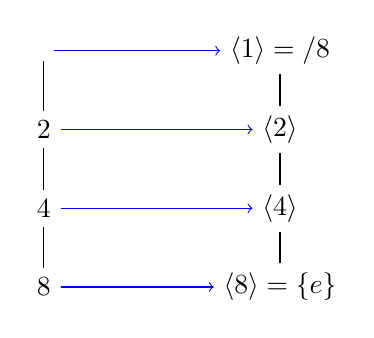
\begin{tikzpicture}
	% end nZ
	\node (z) at (-3,2) {$\Z$};
	\node (2z) at (-3,1) {$2\Z$};
	\node (4z) at (-3,0) {$4\Z$};
	\node (8z) at (-3,-1) {$8\Z$};
	
	\draw (8z) -- (4z);
	\draw (4z) -- (2z);
	\draw (2z) -- (z);
	
	% en Z/nZ
	\node (z8) at (0,2) {$\langle 1 \rangle = \Z/8\Z$};
	\node (z4) at (0,1) {$\langle 2 \rangle$};
	\node (z2) at (0,0) {$\langle 4 \rangle$};
	\node (e) at (0,-1) {$\langle 8 \rangle = \{e\}$};
	
	\draw (e) -- (z2);
	\draw (z2) -- (z4);
	\draw (z4) -- (z8);
	
	% las correspondencias
	\draw (z) edge[->, blue] (z8);
	\draw (2z) edge[->, blue] (z4);
	\draw (4z) edge[->, blue] (z2);
	\draw (8z) edge[->, blue] (e);
	\end{tikzpicture}
	
	\label{fig:reticulo8z}
	\caption{Retículo de subgrupos de $\mathbb{Z}/8\mathbb{Z}$}
\end{figure}

Lo mismo podríamos hacer para obtener el retículo de $\Z/6\Z$ (ver figura \ref{fig:reticulo6z}).

\begin{figure}[h]
	\centering
	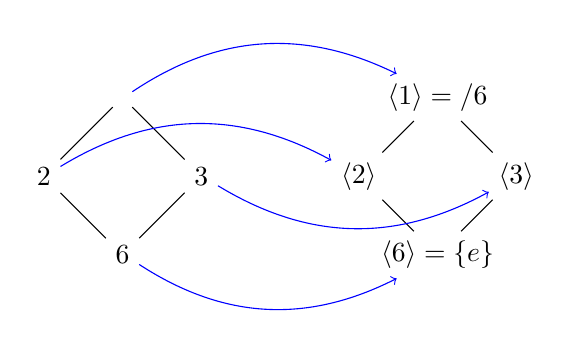
\begin{tikzpicture}
	% en nZ
	\node (z) at (-4, 1) {$\Z$};
	\node (2z) at (-5, 0) {$2\Z$};
	\node (3z) at (-3, 0) {$3\Z$};
	\node (6z) at (-4, -1) {$6\Z$};
	
	\draw (6z) -- (2z);
	\draw (6z) -- (3z);
	\draw (2z) -- (z);
	\draw (3z) -- (z);
	
	% en Z/nZ
	\node (z6) at (0,1) {$\langle 1 \rangle = \Z/6\Z$};
	\node (z2) at (-1,0) {$\langle 2 \rangle$};
	\node (z3) at (1,0) {$\langle 3\rangle$};
	\node (e) at (0,-1) {$\langle 6 \rangle = \{e\}$};
	
	\draw (e) -- (z2);
	\draw (e) -- (z3);
	\draw (z2) -- (z6);
	\draw (z3) -- (z6);
	
	% las correspondencias
	\draw (z) edge[->, bend left, blue] (z6);
	\draw (2z) edge[->, bend left, blue] (z2);
	\draw (3z) edge[->, bend right, blue] (z3);
	\draw (6z) edge[->, bend right, blue] (e);
	
	\end{tikzpicture}
	\label{fig:reticulo6z}
	\caption{Retículo de subgrupos de $\mathbb{Z}/6\mathbb{Z}$}
\end{figure}

\begin{ej}[Retículo de subgrupos de $D_4$]
	Dar el retículo de subgrupos de $D_4 = \{1, B, B^2, B^3, A, AB, AB^2, AB^3\}$, donde $o(A) = 2,\ o(B) = 4,\ BA=AB^3$. En este caso no tenemos más remedio que ir probando a ver qué combinaciones de elementos dan subgrupos. Como conocemos de dónde viene $D_4$ nos es más fácil (ver el ejemplo \ref{ej:famosogrupod4}).

\begin{figure}[h]
	\centering
	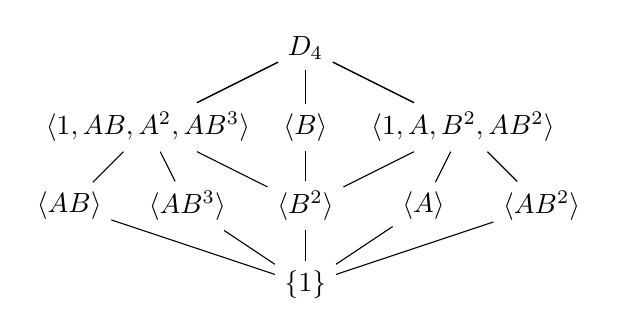
\begin{tikzpicture}
		\node (d4) at (0, 3) {$D_4$};
		\node (1ab) at (-2, 2) {$\langle 1, AB, A^2, AB^3\rangle$};
		\node (b) at (0, 2) {$\langle B \rangle$};
		\node (1ab2) at (2, 2) {$\langle 1, A, B^2, AB^2\rangle$};
		\node (ab) at (-3, 1) {$\langle AB \rangle$};
		\node (ab3) at (-1.5, 1) {$\langle AB^3 \rangle$};
		\node (b2) at (0, 1) {$\langle B^2\rangle$};
		\node (a) at (1.5, 1) {$\langle A \rangle$};
		\node (ab2) at (3, 1) {$\langle AB^2 \rangle$};
		\node (e) at (0,0) {$\{1\}$};
		
		
		\draw (e) -- (ab) -- (1ab) -- (d4);
		\draw (e) -- (ab3) -- (1ab) -- (d4);
		\draw (e) -- (b2) -- (b) -- (d4);
		\draw (e) -- (a) -- (1ab2) -- (d4);
		\draw (e) -- (ab2) -- (1ab2) -- (d4);
		\draw (b2) -- (1ab);
		\draw (b2) -- (1ab2);
	\end{tikzpicture}
	\caption{Retículo de subgrupos de $D_4$}
	\label{fig:reticuloD4}
\end{figure}

\begin{figure}[h]
	\centering
	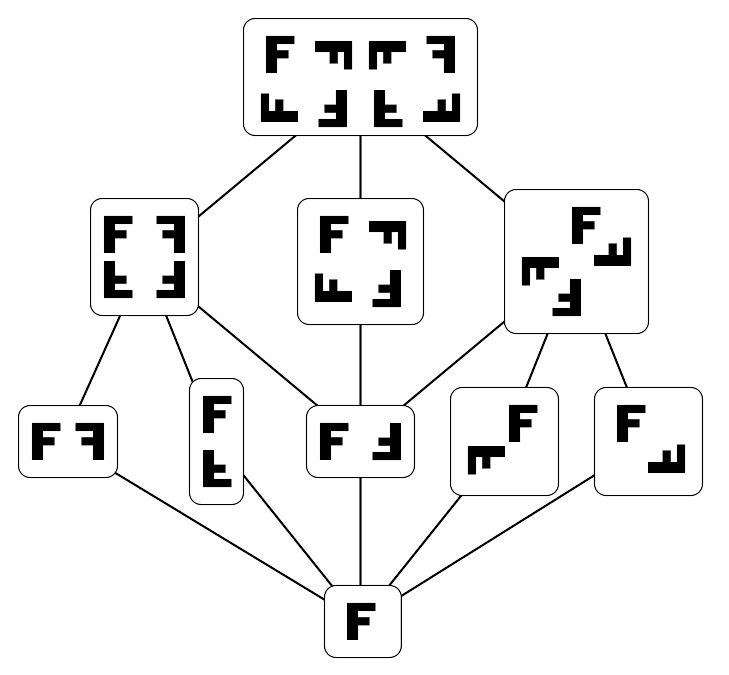
\includegraphics[width=0.25\textwidth]{reticulo-D4}
	\label{fig:reticuloD4dibujo}
	\caption{Retículo de subgrupos de $D_4$ de \cite{d4sub}}
\end{figure}
	
	\textit{Nos ayudamos de la imágen para sacarlos. La manera de hacerlo sin tener más información que la presentación del grupo es hacerse todos los subgrupos generados por cada elemento y descartar los que son iguales. Luego hacerse todos los subgrupos generados por dos elementos y descartar los que son iguales. Por alguna razón no hace falta probar con los generados por más de dos elementos. Una vez obtenidos estos grupos establecemos las relaciones de inclusión y creamos el diagrama de Hasse.}
\end{ej}

\begin{ej}
	Retículo de subgrupos del grupo de cuaterniones $H$ (figura \ref{fig:reticulocuaterniones})
	
	\begin{figure}[h]
		\centering
		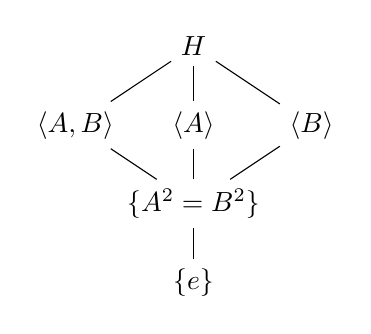
\begin{tikzpicture}
		\node (H) at (0,3) {$H$};
		\node (ab) at (-1.5, 2) {$\langle A, B\rangle$};
		\node (a) at (0,2) {$\langle A \rangle$};
		\node (b) at (1.5,2) {$\langle B \rangle$};
		\node (b2) at (0,1) {$\{A^2 = B^2\}$};
		\node (e) at (0,0) {$\{e\}$};
		
		\draw (e) -- (b2) -- (a) -- (H);
		\draw (b2) -- (ab) -- (H);
		\draw (b2)-- (b) -- (H);
		\end{tikzpicture}
		\caption{Retículo de subgrupos del grupo de cuaterniones $H$.}
		\label{fig:reticulocuaterniones}
	\end{figure}
\end{ej}

\begin{ej}[Retóculo de subgrupos de $D_5$]
	\label{ej:reticulod5}
	\begin{figure}
		\centering
		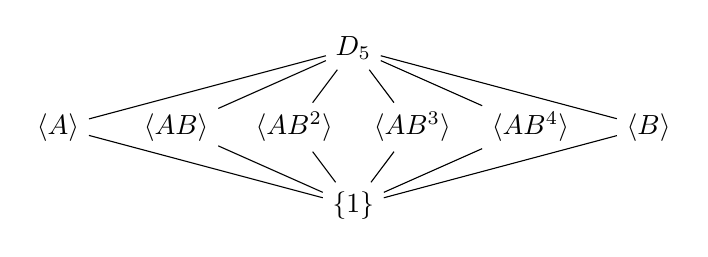
\begin{tikzpicture}
			\node (d5) at (0,2) {$D_5$};
			\node (a) at (-3.75, 1) {$\langle A \rangle$};
			\node (ab) at (-2.25, 1) {$\langle AB \rangle$};
			\node (ab2) at (-0.75, 1) {$\langle AB^2 \rangle$};
			\node (ab3) at (0.75, 1) {$\langle AB^3\rangle$};
			\node (ab4) at (2.25, 1) {$\langle AB^4\rangle$};
			\node (b) at (3.75, 1) {$\langle B \rangle$};
			\node (e) at (0,0) {$\{1\}$};
			
			\draw (e) -- (a)   -- (d5);
			\draw (e) -- (ab)  -- (d5);
			\draw (e) -- (ab2) -- (d5);
			\draw (e) -- (ab3) -- (d5);
			\draw (e) -- (ab4) -- (d5);
			\draw (e) -- (b)   -- (d5);
		\end{tikzpicture}
		\caption{Retículo de subgrupos de $D_5$.}
	\end{figure}
\end{ej}



\section{Construcción de homomorfismos e isomorfismos de grupos}

Sea $G$ abeliano con $|G| = n = rs$, sea $H < G,\ K < G$ con $|H| = r,\ |K| = s$ y $H\cap K = \{e\}$.
\begin{itemize}
	\item Notemos que como $G$ es abeliano, $H$ y $K$ son subgrupos normales.
	\item Al aplicar el teorema $\ref{thm:cardinalidadproductolibre}$ tenemos que el denominador es $|H\cap K| = 1$ por lo que $|HK| = |H| |K| = rs= n$.
	\item Como $G$ es abeliano:
	\begin{enumerate}
		\item $G = HK$ (porque $HK$ es un subgrupo con el mismo número de elementos que $G$ por el teorema \ref{thm:cardinalidadproductolibre})
		\item La función $f:H\times K \to G,\ (h, k)\mapsto hk$ es un homomorfismo de grupos (nótese que esto no ocurriría si $G$ no fuese abeliano).
	\end{enumerate}
\end{itemize}

Es más, si se cumple todo lo anterior, $f$ es además un isomorfismo $\implies H\times K \isom G$.

\begin{ej}[Homomorfismo trivial]Siempre nos queda el homomorfismo trivial $f:G_1 \to G_2,\ f(g_1) = e_2, \forall g_1 \in G_1$.
\end{ej}

\begin{ej}
	\label{ej:nohomoentreproducto}
	Consideramos $S_3$, que tiene $|S_3| = 6$ y no es abeliano y los subgrupos $H = \langle (12) \rangle$ y $K = \langle (123) \rangle$ con $|H| = 2$ y $|K| = 3$. Podemos construir la función $f:H\times K \to S_3$ pero no es un homomorfismo de grupos. De hecho, al ser $K \normsub S_3$, el producto $HK$ es un subgrupo y la función $f$ es una biyección, pero aún así no es compatible con la estructura de grupo.
\end{ej}

\begin{ej}
	Consideramos $D_4$ y un grupo $G$ con $a,b \in G$ donde hemos establecido un homomorfismo que definimos con $f(A) = a$ y $f(B) = b$. Ocurre lo siguiente
	\begin{itemize}
		\item El homomorfismo queda totalmente definido ya que todos los elementos de $D_4$ son palabras en $A$ y $B$ y por la estructura de homomorfismo podemos operar tras aplicar la operación a cada letra. Por ejemplo $f(ABA) = aba$.
		\item Es necesario que $o(a) = 2$ y $o(b) = 4$, de lo contrario no se cumpliría la estructura de homomorfismo entre $D_4$ y $G$.
	\end{itemize}
\end{ej}

\begin{ej}
	Consideramos $\ZnZ = \{0, 1, \dots, n-1\}$ La presentación de este grupo es $o(1) = n$. Queremos construir un homomorfismo $f:\ZnZ \to G'$. Para que $f$ sea un homomorfismo necesitamos que $f(0) = e$. Ahora supongamos que establecemos $f(1) = a$. Naturalmente sigue (para que $f$ sea un homomorfismo) que $f(2) = a\ast a = a^2$. Observamos que la condición necesaria y suficiente para que el homomorfismo definido por $f(1) = a$ es que $a^n = e$, o lo que es lo mismo que $o(a)$ divida a $n$.
	\begin{align*}
	f:\ZnZ &\to G' \\
	0 &\mapsto e \\
	1 &\mapsto a \\
	2 &\mapsto a^2\\
	&\dots \\
	n = 0 &\mapsto a^n = 0
	\end{align*}
\end{ej}

\begin{ej}
	En $\ZnZ \to \ZnZ$ podemos construir $n$ homomorfismos ya que
	\begin{itemize}
		\item cualquier $a \in \ZnZ$ es cumple la condición necesaria para que $f(1) = a$ induzca un homomorfismo
		\item todo homomorfismo queda determinado por $f(1) = a$ para algún $a \in \ZnZ$.
	\end{itemize}
	
	Es decir que $\text{Hom}(\ZnZ, \ZnZ) \isom \ZnZ$.
\end{ej}

\begin{ej}
	Si ahora nos preguntamos por los isomorfismos $\text{Isom}(\ZnZ, \ZnZ) \subset \text{Hom}(\ZnZ, \ZnZ)$ nos damos cuenta de que los únicos $a \in \ZnZ$ que nos dan isomorfismos son aquellos que tienen $o(a) = n$.
	
	Es decir que $\text{Isom}(\ZnZ, \ZnZ) \isom \uds{\ZnZ}$.
\end{ej}

\begin{ej}[Isomorfismo conjugación]
	Fijamos $g \in G$ y definimos $\phi_g:G \to G,\ x \mapsto gx\inv{g}$. Es un homomorfismo de grupos pues $y\mapsto gy\inv{g}$ y $xy \mapsto gxy\inv{g} = gx\inv{g}gy\inv{g}$.
	
	Ahora consideramos $\inv{g}$ y $\phi_{\inv{g}}: G \to G,\ x \mapsto \inv{g}xg$ y como antes se verifica que es homomorfismo.
	
	Además, $\phi_g \circ \phi_{\inv{g}} = id$ luego $\phi_g$ es un isomorfismo de grupos.
\end{ej}


\begin{ej}
	Consideramos ahora $N \normsub G$ y por tanto para cualquier $g \in G,\ gN = Ng$. La función $\phi_g(N) \subset N$ es un isomorfismo que además lleva los elementos de $N$ en $N$, por tanto podemos restringirla a $\phi_g:N \to N$ e inducir un isomorfismo.
	
	Es decir, los subgrupos que no se mueven por ninguna función $\phi_g$ son los subgrupos normales.
\end{ej}

\begin{ej}
	Consideramos el grupo $(\Z, +)$ que es cíclico y un grupo $G$ con $a \in G$. Utilizando notación multiplicativa en la que el $\mathbf{1}$ representa el elemento neutro (en este caso $\mathbf{1} = 0$)
	\begin{align*}
	\Z &\to G \\
	\mathbf{1} &\mapsto a \\
	k &\mapsto a^k \\
	k + k' &\mapsto a^{k+k'}
	\end{align*}
	Es decir, que al seleccionar $\mathbf{1} \mapsto a$ queda determinada la imágen de todos los demás $k \in \Z$ y además la función que obtenemos es un homomorfismo. Por tanto el conjunto de los homomorfismos de $\Z$ en $G$ es TODO $G$: $\text{Hom}(\Z, G) = G$.
\end{ej}

\begin{ej}[del primer teorema de la isomorfía]
	Consideramos el grupo $G = \{1, i, -1, -i\}$ con el producto y establecemos la función $f:\Z \to G$ que lleva $1 \mapsto i$. Además $f$ es sobreyectiva y $\ker f = \Z/4\Z$. El primer teorema de la isomorfía nos dice que existe un isomorfismo $\overline{f}: \Z/\ker f \to G$ y este es $\overline{f},\ \overline{f}([a]) \mapsto i^{a}$ (en $\ker f$ no se repiten los elementos por lo que convertimos el epimorfismo $f$ en un homomorfismo $\overline{f}$).
\end{ej}

En general todos los grupos cíclicos de orden $n$ son isomorfos entre sí, porque todos son isomorfos a $\Z/n\Z$ y los isomorfismos son reversibles y la composición sigue siendo isomorfismo.

Hemos visto que $\text{Hom}(\Z, G) = G$ porque al determinar $f(1) = a$ determinamos el homomorfismo y por tanto tenemos un homomorfismo para cada elemento $a \in G$.

¿Pero qué pasa si tomamos los homomorfismos $f:\ZnZ \to G$ con $a \in G$ definidos por $f(\overline{1}) = a$? Pasa que para que sean homomorfismos necesitamos que $o(a) = o(1) = n$ para que así $\overline{0} = \overline{n} \mapsto a^n = e$.

\begin{ej}
	Veamos un ejemplo (notamos que $(12)^4 = id$)
	\begin{align*}
	f:\Z/4\Z &\to S_3 \\
	\overline{1} &\mapsto (12) \\
	\overline{2} &\mapsto id = (1) \\
	\overline{3} &\mapsto (12) \\
	\overline{4} = \overline{0} &\mapsto id
	\end{align*}
	
	Observamos que $\text{Hom}(\Z/4\Z, S_3) \subset \text{Hom}(\Z, S_3)$ puesto que al tomar $\Z/4\Z$ no podemos tomar cualquier $a$ sino que tenemos que asegurarnos de que $o(a) = o(1)$ (en este caso $o(a) = 2$ pero sigue funcionando porque lo que importa es que $a^{o(1)} = id$).
\end{ej}

Queremos analizar los homomorfismos $f:\ZnZ \to \ZnZ$. Ahora no importa el $\overline{a}$ que elijamos para que $f$ sea homomorfismo porque $\ima f = \langle \overline{a} \rangle$. 

Para que $f$ sea epimorfismo, necesitamos que $\ima f = \langle \overline{a} \rangle = \ZnZ$ es decir que $o(a)$ sea coprimo con $n$.

Concluímos que $\text{Aut}(\ZnZ) \subset \text{Hom}(\ZnZ, \ZnZ)$.

